\chapter{Detailed Project Schedule}\label{app:schedule}
\section{Timeline and Scheduling Assumptions}
This schedule reflects work recorded by 30 October 2026. September and October tasks are supported by repository evidence; later dates are proposed milestones, subject to the official FYP calendar. Ghada leads V3 editorial/verification and scheduling/database engineering. Aya leads acquisition and performance/reliability measurement. Joud leads frontend implementation and briefing-quality/user evaluation, including target users, human reference review, split stewardship and English/French/Arabic assessment. Integration and security remain shared responsibilities. Ownership identifies accountability, not exclusive authorship.

\begin{figure}[H]\centering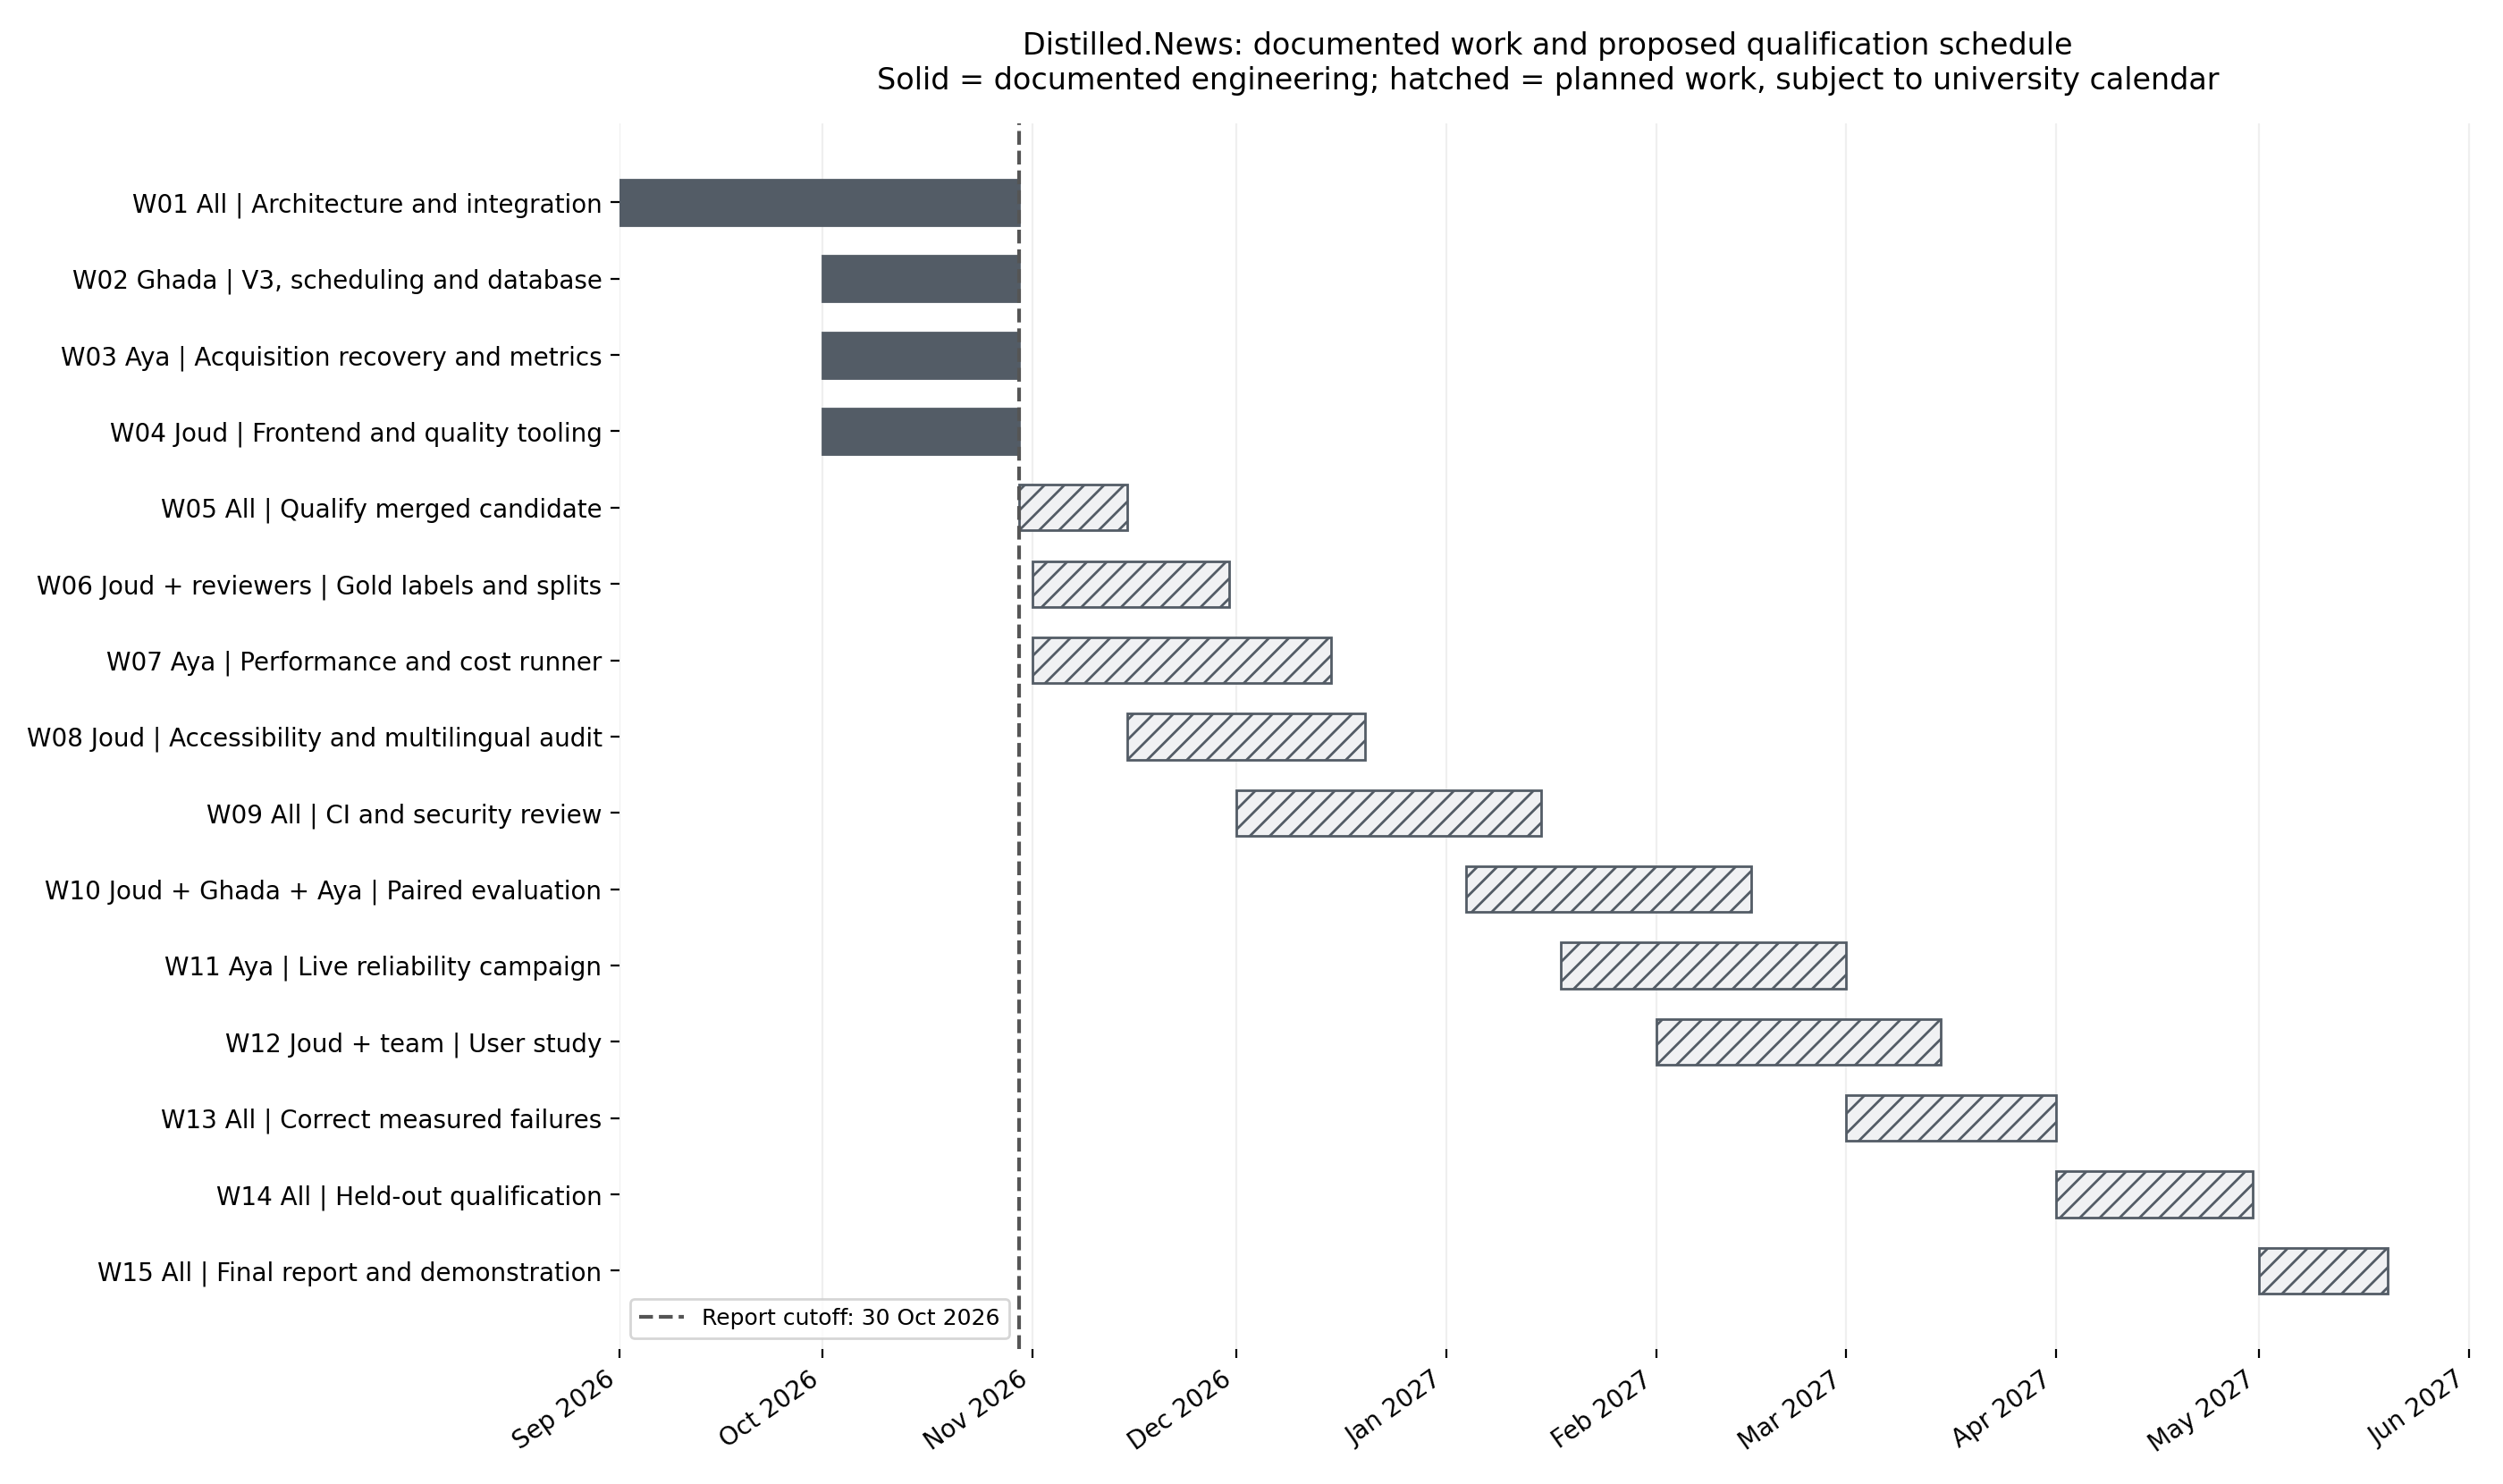
\includegraphics[width=.85\textwidth]{Figures/gantt.png}\caption{Owner-labelled Gantt schedule. Filled bars show documented September and October work. Hatched bars indicate planned work; the vertical line marks this report date. Planned dates require confirmation against the university calendar.}\label{fig:gantt}\end{figure}

\section{Detailed Work Breakdown, Dependencies and Milestones}
\small
\begin{longtable}{L{1.1cm}L{2.45cm}L{3.95cm}L{2.2cm}L{3.1cm}}
\caption{Team schedule with test gates and deliverable dates}\label{tab:schedule}\\\toprule ID & Target period / owner & Work package & Dependency & Exit evidence / milestone \\ \midrule\endfirsthead\toprule ID & Period / owner & Work package & Dependency & Exit evidence \\ \midrule\endhead
W01 & Sep--Oct 2026; all & Define architecture, interfaces, source acquisition and downstream pipeline & Approved initial scope & Dated development records, implementation docs and staged integration (completed) \\
W02 & Oct 2026; Ghada & V3 editorial implementation, targeted repair, QA replay, prompt trials & W01 & Native output, ledger receipts, negative-case analysis (completed/ongoing) \\
W03 & Oct 2026; Aya & Source integration, recovery and performance metric definition & W01 & Implementation and offline calculation-test evidence (completed/ongoing) \\
W04 & Oct 2026; Joud & Frontend/mail/PWA integration and multilingual quality-review tooling & W01 & Integrated interface and local tooling; human quality labels pending \\
W05 & Oct 30--Nov 15; all & Integrated candidate available; qualify integration, finalize requirements and quality labels & W02--W04 & Integration manifest and no unresolved critical ownership/migration defects \\
W06 & Nov 1--30; Joud + reviewers; Ghada supports & Review real source/coverage labels; certify splits and independent second review & W05 & Frozen source hashes, event IDs, judge guide and disagreements \\
W07 & Nov 1--Dec 15; Aya & Build opportunity manifest, end-to-end timing/cost collectors and baseline adapters & W05 & Reproducible runner and timestamp-contract tests \\
W08 & Nov 15--Dec 20; Joud & Accessibility and multilingual UI regression suite, notification receipt instrumentation & W05 & Browser, keyboard and RTL audit; client-receipt caveats \\
W09 & Dec 1--Jan 15; all & CI/CD and DevSecOps: secret/dependency scans, migration dry run, environment protection, provenance, rollback & W05 & Passing checks, staged release gate and failure artifacts \\
W10 & Jan 4--Feb 15; Joud + Ghada + Aya & Per-language quality comparisons; chronology/repair faults and performance analysis & W06,W07 & Per-language quality/latency/cost with independent labels and CIs \\
W11 & Jan 18--Mar 1; Aya & Controlled live windows, queue/provider fault injection and ledger reconciliation & W07,W09 & Offered-opportunity outcomes, deadline-SLO and failure report \\
W12 & Feb 1--Mar 15; Joud + all & Consent-based user monitoring pilot and task comparison & W06,W08 & Time/source-opening distributions, interviews, limitations \\
W13 & Mar 1--Apr 1; all & Correct top measured failure modes without weakening safety gates & W10--W12 & Frozen A/B replays and regression evidence \\
W14 & Apr 1--30; all & Final qualification on held-out and controlled live cases & W13 & Release acceptance matrix with failed/unknown cells reported \\
W15 & May 1--20; all & Final report, demonstrations, reproducibility package and oral defense & W14 & Final implementation, documentation, demo and supervisor review \\
\bottomrule\end{longtable}
\normalsize

\newpage
\section{Critical Path and Risk Buffer}
The critical path is \textbf{integrated-system qualification $\rightarrow$ frozen independent labels $\rightarrow$ comparable evaluation harness $\rightarrow$ controlled QA $\rightarrow$ final acceptance}. UI refinements and supplementary acquisition adapters may proceed concurrently, but they cannot substitute for this path. We reserve the second half of March for measured defect correction and April for held-out requalification; a late model or prompt change reopens the corresponding gate. Critical authorization or unsupported-fact failures block publication promotion regardless of an attractive aggregate speed score.

\section{Team Coordination and Review Cadence}
We propose one weekly 30-minute engineering coordination session, with a shared agenda listing blocker, owner, changed requirement, next experiment, permitted expense and agreed due date. A separate weekly pull-request/release review inspects CI evidence, migration compatibility and negative test cases. Each formal meeting should record actual date, attendance, decisions and action closure. Appendix C separates weekly evidence-backed engineering checkpoints from formal meeting minutes, which require actual attendance and decisions.
